%%% template.tex
%%%
%%% This LaTeX source document can be used as the basis for your technical
%%% paper or abstract. Intentionally stripped of annotation, the parameters
%%% and commands should be adjusted for your particular paper - title, 
%%% author, article DOI, etc.
%%% The accompanying ``template.annotated.tex'' provides copious annotation
%%% for the commands and parameters found in the source document. (The code
%%% is identical in ``template.tex'' and ``template.annotated.tex.'')

\documentclass[annual, 12pt]{acmsiggraph}
\usepackage{program}

\TOGonlineid{45678}
\TOGvolume{0}
\TOGnumber{0}
\TOGarticleDOI{1111111.2222222}
\TOGprojectURL{}
\TOGvideoURL{}
\TOGdataURL{}
\TOGcodeURL{}

\title{Mobile Depth from Focus and Applications}

%\author{Naran Bayanbat\thanks{e-mail:naranb@stanford.edu}\\Stanford University \and Jason Chen\thanks{e-mail:jasonch@stanford.edu} \\Stanford University \and Chun-Wei Lee\thanks{e-mail:chunweil@stanford.edu} \\Stanford University}
\author{Naran Bayanbat\\naranb@stanford.edu\\Stanford University \and Jason Chen\\jasonch@stanford.edu\\Stanford University \and Chun-Wei Lee\\chunweil@stanford.edu\\Stanford University}
\pdfauthor{Naran Bayanbat, Jason Chen, Chun-Wei Lee}

\keywords{depth from focus, depth map, tablet, computational photography}

\begin{document}

 \teaser{
   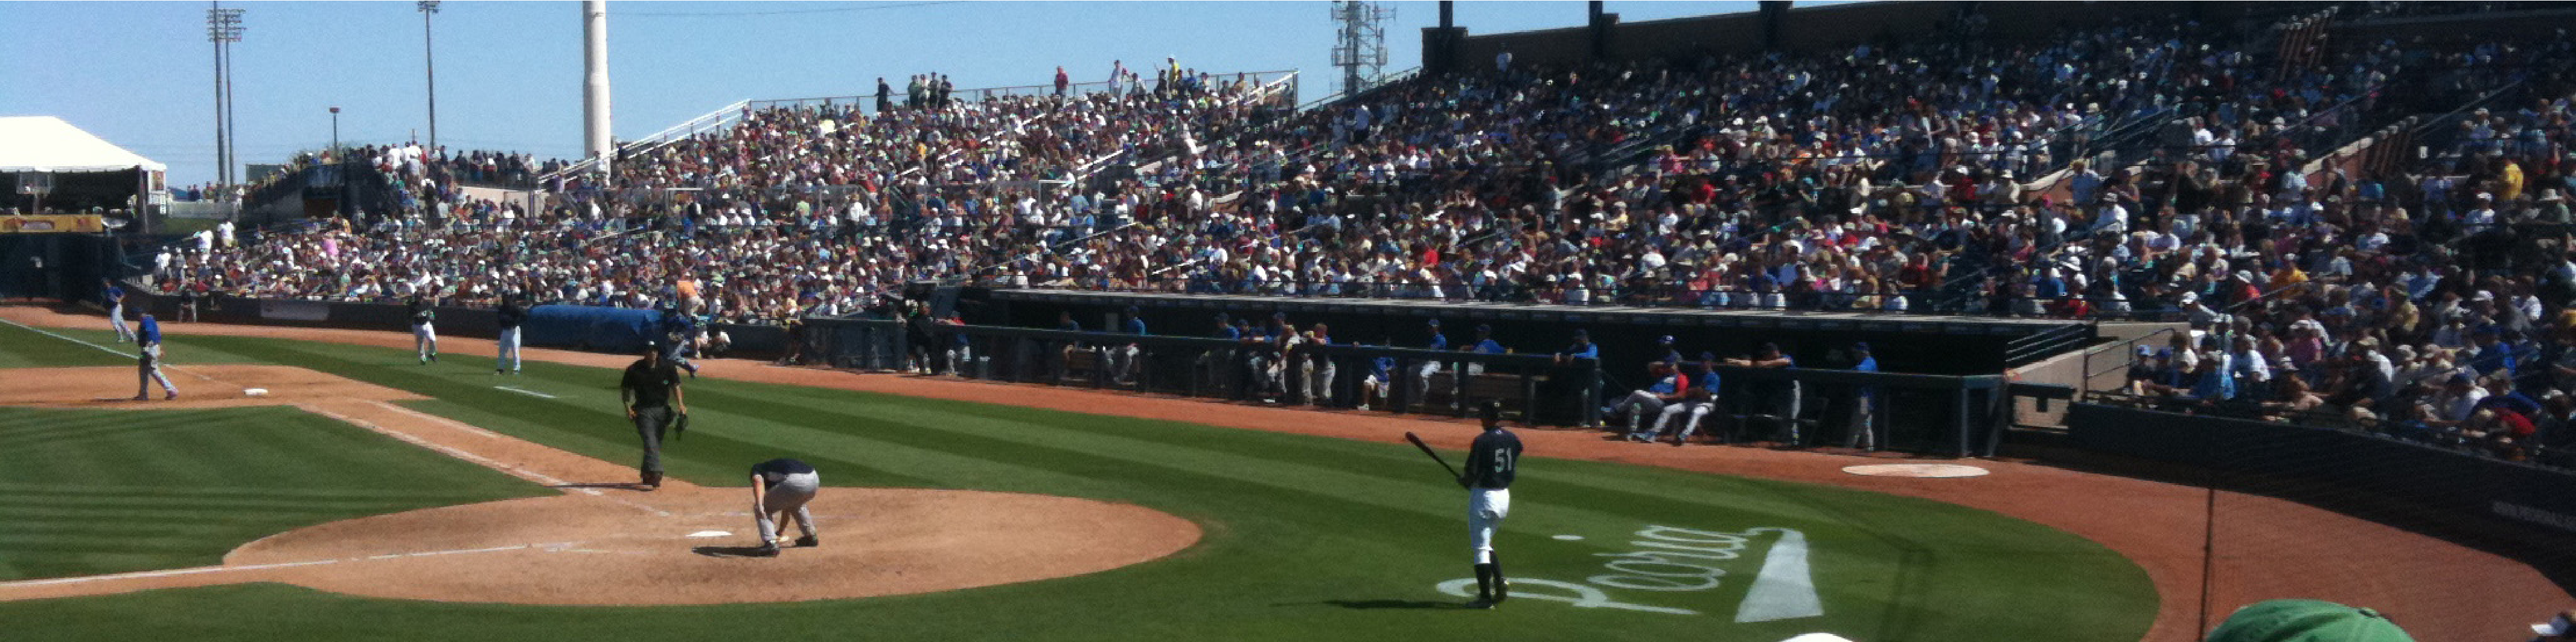
\includegraphics[height=1.5in]{images/sampleteaser}
   %\caption{}
 }

\maketitle

\begin{abstract}
Depth information is crucial in providing scene understanding for many post-processing applications in computational photography. While depth maps can be easily obtained through stereo cameras or external devices such as infrared sensors, it is difficult in mobile photography because of hardware limitation. In this project, we will implement depth-by-focus, sweeping a single lens across various focus distances and composite an approximate depth map. The depth map will be improved by segmentation and bilateral filtering. We will then demonstrate the effectiveness of the technique by utilizing the depth map and simulate light-field photography as well as synthetic depth of field.

\end{abstract}

\begin{CRcatlist}
  %\CRcat{I.3.3}{Computer Graphics}{Three-Dimensional Graphics and Realism}{Display Algorithms}
  %\CRcat{I.3.7}{Computer Graphics}{Three-Dimensional Graphics and Realism}{Radiosity};
\end{CRcatlist}

\keywordlist

%\TOGlinkslist

\copyrightspace

\section{Introduction}

Mobile devices have become the most common photography means, and they have presented a new set of opportunities and challenges for computational photography.  While many applications take advantage of these devices' location, accelerameter, and other meta data, the inherent hardware limitation on size computation power makes it worth revisiting prior works on computational photography to this application.  Specifically, since depth information is one of the most useful piece of scene understanding, we wish to demonstrate a mobile solution producing a depth map that assist in computational photography.  Since most mobile devices have only one camera (lens) and no active focusing equipment, we will attempt to implement depth from focus, approximating depth information from images captured at different depths. 

\section{Prior Work}

Depth from Focus is a technique that has been studied for decades \cite{Grossmann1987} \cite{pyramid} and with numerous applications, as it is relatively easy to compute and implement and requires no additional hardware.  It is also flexible and can be adjusted for real-time, low resolution depth map \cite{mobileRobot} as well as more detailed depth maps.

\section{Results}

\subsection{Depth Sampling}
At each focus distance, we densely sampled 36x27 square patches of width 30 pixels and calculate the sharpness of each patch.  We tried many different sharpness measures, starting with a simple high pass filter to the Sobel edge detection filter.  After evaluating the results, we concluded Sobel edge detection filter produces the best results. Sobel filter is composed of the horizontal box filter, $G_x$, and the vertical box filter, $G_y$, which are 
\[
G_x = \begin{bmatrix} -1 & 0 & 1 \\ -2 & 0 & 2 \\ -1 & 0 & 1 \end{bmatrix}
G_y = \begin{bmatrix} -1 & -2 & -1 \\ 0 & 0 & 0 \\ 1 & 2 & 1 \end{bmatrix}
\]. For each pixel in the image at $(i,j)$, we compute its sharpness value $l_{x,y}$ as 
\begin{eqnarray}
gx &:=& G_x * I_d[i,j] \nonumber \\
gy &:=& G_y * I_d[j,i] \nonumber \\
l_{i,j} &:=& gx^2 + gy^2 
\end{eqnarray}, where $gx$ is the resulting value after applying the Sobel horizontal box filter, and $gy$ the vertical box filter. Finally, the sharpness $\lambda_{x,y}$ to be the sum of all pixel sharpness $l$ within the patch. \\
As we sweep across different focus distances, we record only the current maximum sharpness and the focus distance at which this is obtained for each sample point. We make the assumption that an object exists at the distance which produces the maximum sharpness response.  Prior works have attempted to interpolate the response curve and estimate the true maximum \cite{Grossmann1987}, but we decided this is unnecessary for our applications and too much computation on a mobile device. 

\subsection{Depth Map Generation}
\label{sec:depthmap-generation}
One of the inherent problem in sharpness calculations, as well as in all focusing methods in general, is that they fail on textureless surfaces.  Therefore, after obtaining the best focus distance and best sharpness pair, $<d_i, \lambda_i>$, for each sample point, we first correct for points sampled at low texture patches.  Every sample point whose sharpness is below some predefined threshold, $\Lambda$, will update its sharpness by finding the most common depth value in the patches around it.  This is achieved by a simple voting scheme: each of the nine pixels will cast a vote for the depth value it represents, and its vote is weighted by its confidence, which is the normalized sharpness value. \\

Then, we simply naively assume the entire patch exists at the same depth, thus generating a blocky depth map as in Figure ~\ref{fig:initial-depth-map} of the same dimension as the input image. Next, we take a full-colored frame from the input stack as reference image, and use joint bilateral filtering to smooth out the patch boundaries.  This is because we want fairly aggressive smoothing while preserving edges from the color space. \\
This gives us our first approximate depth map, as shown in Figure ~\ref{fig:filtered-depth-map}.  We quickly realized that any frame we could choose from the stack could not serve as a good edge reference, because at least some part of the image is out of focus.  We can solve the problem if we had an all-in-focus image, but we could only get a good all-in-focus image if we had a better depth map.  To solve this problem, we iteratively refined our depth map by generating all-in-focus image based on the current depth map (Figure ~\ref{fig:depth-map-refining}).  This provides us highly accurate depth map with clear object edges, while smoothing the borders to produce convincing transition between the patches, Figure ~\ref{fig:refined-depth-map}.
\begin{figure}
\centering
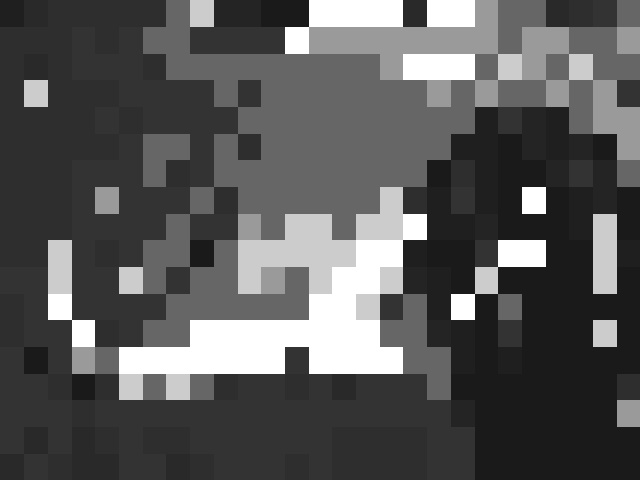
\includegraphics[height=1.5in]{images/initial-depth-map.jpg}
\caption{Initial Depth Map}
\label{fig:initial-depth-map}
\end{figure}

\begin{figure}
\centering
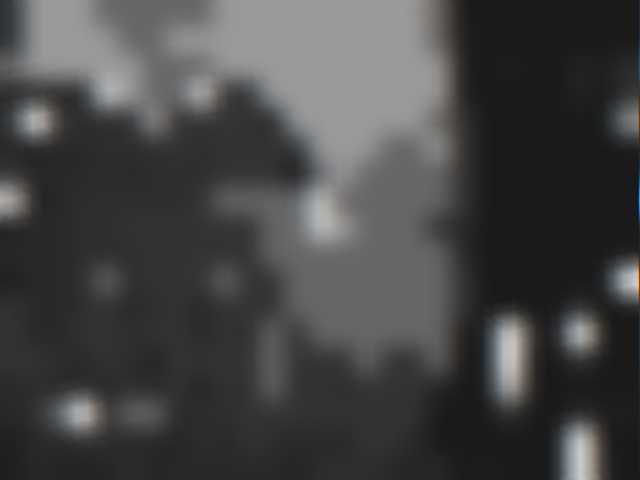
\includegraphics[width=3in]{images/filtered-depth-map.jpg}
\caption{Depth Map Filtered with Bilateral Filtering}
\label{fig:filtered-depth-map}
\end{figure}

\begin{figure}
\centering
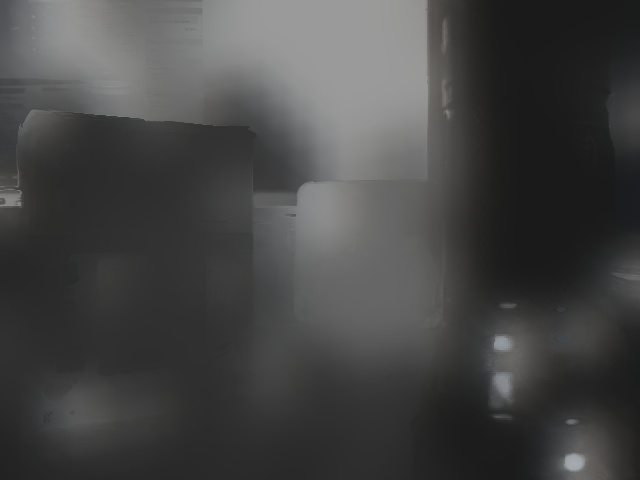
\includegraphics[width=3in]{images/refined-depth-map.jpg}
\caption{Depth Map Refined with All-in-Focus Image once}
\label{fig:refined-depth-map}
\end{figure}

\begin{figure}
\centering
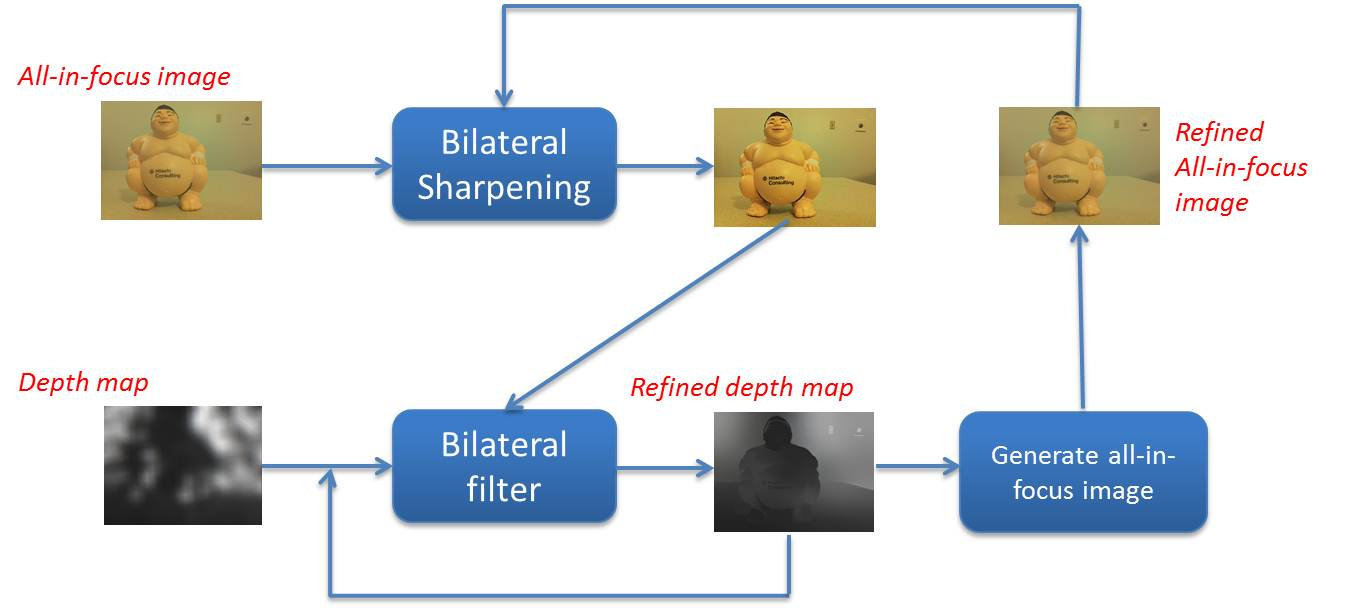
\includegraphics[width=3in]{images/depth-map-refining.jpg}
\caption{Depth Map Refining with All-in-Focus Images}
\label{fig:depth-map-refining}
\end{figure}

\subsection{All-in-Focus Imaging}

One application of having an image stack and an approximate depth map is to produce all-in-focus images.  As mentioned in section ~\ref{sec:depthmap-generation}, an all-in-focus image can also be used to further improve our depth map.  The algorithm to generate all-in-focus images is simple and intuitive.  For each pixel on the final image, we simply sample from the image in the stack as indicated by the closest depth value. I.e., for each pixel $p_{i,j}$, 
\begin{equation} 
p_{i,j} := images[ depthmap_{i,j} ](i,j)
\end{equation}, where images is image stack represented as an array, and depthmap returns values which are indices into the array.  
\subsubsection{Calibration}

\begin{figure}
\centering
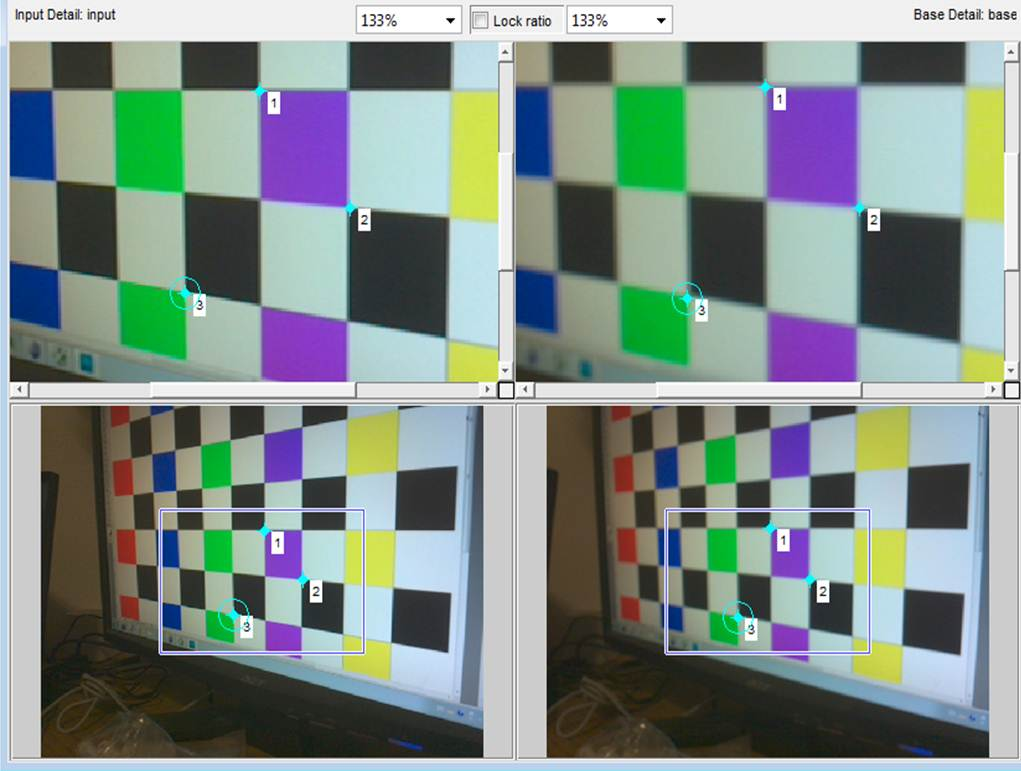
\includegraphics[width=3in]{images/calibration.jpg}
\caption{Calibration Image}
\label{fig:calibration}
\end{figure}

There is a subtle problem to solve when merging images at different focus distances: each focus distance has a slight optical magnification.  Images taken at closer focus distances will be magnified by an amount that is dependent on each lens' manufacturing specification.  Fortunately, since this geometric distortion is consistent across all images taken by the same camera, we can calibrate once just once and store the transformation matrices statically. We use calibration images Figure ~\ref{fig:calibration} and hand-label control points that are corresponding in each pair of images. Since this is a non-reflective similarity transform, only two pairs of control points are necessary for each pair of images.  We compute the transformation matrices using the image with the smallest focus distance as base image.  This is because any coordinate in this image will have a correspondence in farther-focused images, but not vice versa.  Each transformation matrix, $C_d\in R^{3x3}$, transforms homogenized target image coordinates $(x,y,1)$ to the coordinates in the image captured at depth $d$, $(x_d,y_d,1)$. So now we revise the equation to be
\begin{eqnarray} 
v &:=& [x,y,1] \nonumber \\
d &:=& depthmap_{i,j}  \nonumber \\
p_{i,j} &:=& images[ d ]( (C_d v)_x, (C_d v)_y)
\end{eqnarray}. The resulting all-in-focus images are in fact very convincing, as seen in figure ~\ref{fig:all-focus-calibrated}.

\begin{figure}
\centering
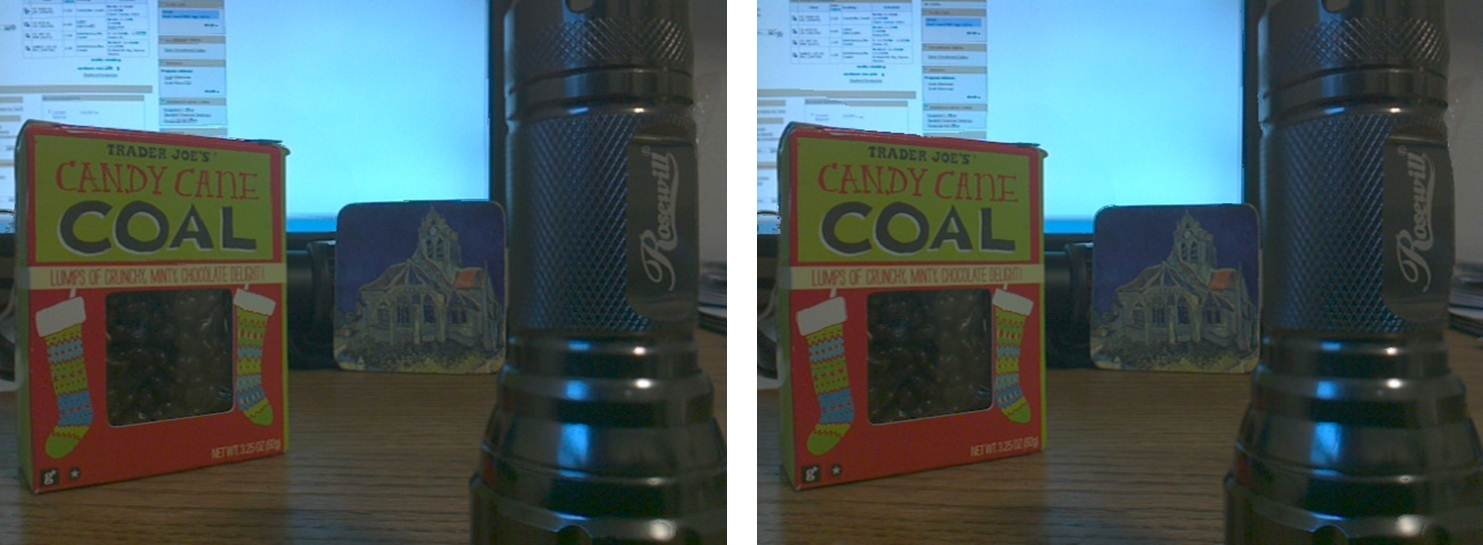
\includegraphics[width=3in]{images/all-focus-calibrated.jpg}
\caption{Comparing all-in-focus images before calibration (right) and after (left). Notice the curve on the flashlight's edge on the right is corrected.}
\label{fig:all-focus-calibrated}
\end{figure}


\subsection{Synthetic Depth of Field Application}

A reverse application of an all-in-focus image would be to create images with synthetic depth-of-field effect. A common use of this would be to create an artificial shallow depth-of-field in an image for artistic effect. Yet another application would be to create the "miniature model" effect in images, to create the look and feel of a smaller scene than the one present in reality. Fortunately, we can leverage on the information provided by the DOF map to generate a realistic looking DOF. 

Our synthetic DOF application requires an all-in-focus image as well as a DOF map. Given these two, we can accept any arbitrary focal length, and generate an image with an "accurate" amount of blur (since we do not model some effects of focal length change, such as magnification,  the generated is not hundred percent accurate. Furthermore, we can certain assumptions, such as circular aperture, that make the synthetic blurring process simpler) (make this footnote?). We use the following equation to calculate the appropriate blur radius $R$ of a pixel, given the new focal length: 

\begin{eqnarray} 
R=s\frac{D}{2}[\frac{1}{f}-\frac{1}{u}-\frac{1}{s}]
\end{eqnarray}

where $f$, $u$, $s$, and $D$ are the new focal length, the distance to object from lens, the distance to the image plane from lens, and the lens diameter, respectively (Murali Subbarao). Here, $s$ and $D$ are camera specific constants. Now, let us use the depth field information. Given the depth field, for each pixel, we can estimate the focal length that gives us a zero blur radius: 

\begin{eqnarray} 
0 &=& s\frac{D}{2}[\frac{1}{f_{0}}-\frac{1}{u}-\frac{1}{s}], which results in\nonumber \\
\frac{1}{s} &=& \frac{1}{f_0} - \frac{1}{u} 
\end{eqnarray}

Here, $f_0$ denotes the zero blur focal length. We can now simplify the initial expression to for blur radius:

\begin{eqnarray} 
0&=&s\frac{D}{2}[\frac{1}{f_{0}}-\frac{1}{u}-\frac{1}{s}], which results in \nonumber \\
\frac{1}{s}&=&\frac{1}{f_{0}}-\frac{1}{u} 
\end{eqnarray}

\begin{eqnarray} 
R &=& s\frac{D}{2}[\frac{1}{f}-\frac{1}{f_0}], or \nonumber \\
R &\propto& \frac{1}{f}-\frac{1}{f_{0}}
\end{eqnarray}
 
Since $s$ and $D$ are intrinsic constants of the camera, we are not interested in them. Furthermore, in our application, we wish allow the users to customize the degree of synthetic blur. Consequently, we do not require calibration to measure $D$ and $s$. 

\begin{figure}
\centering
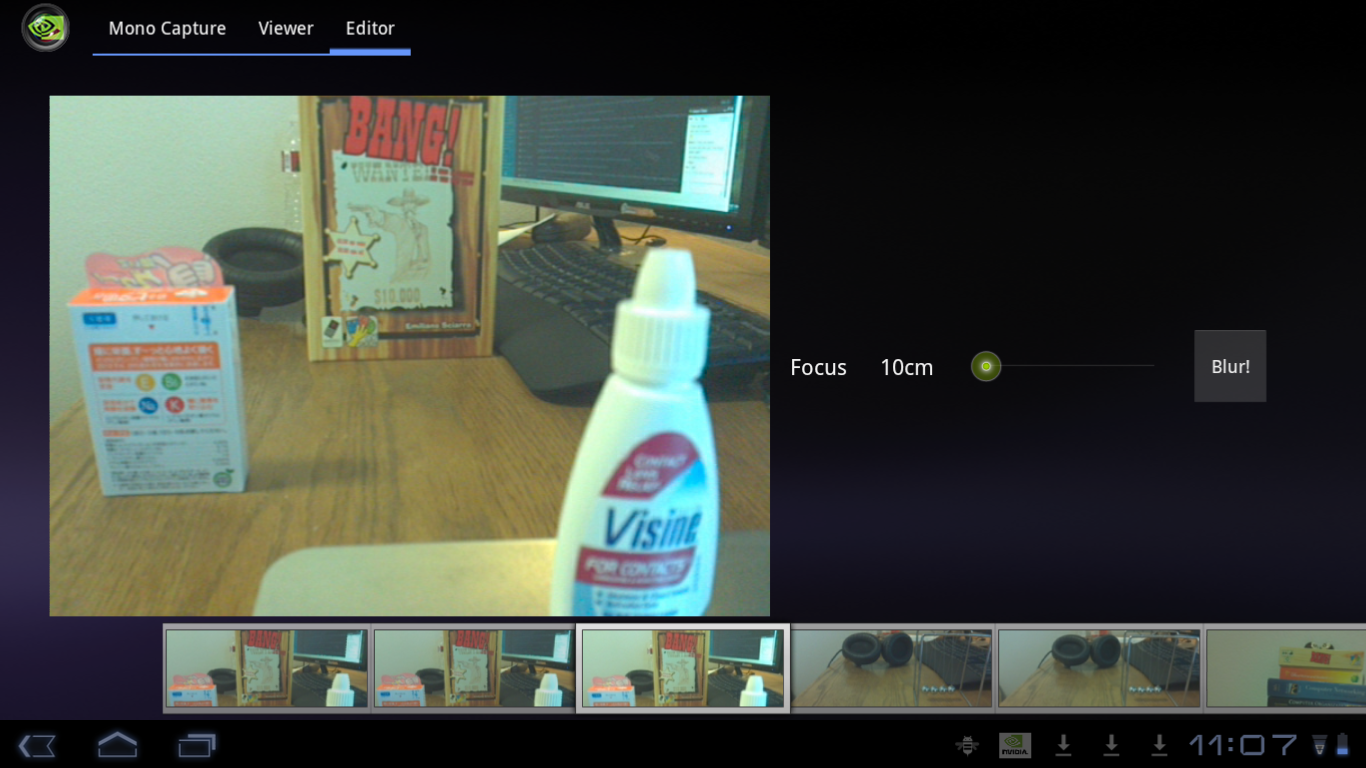
\includegraphics[width=3in]{images/synthetic-blur-screenshot.png}
\caption{Screen Shot of Synthetic Blur App}
\label{fig:synthetic-blur-shot}
\end{figure}

To generate an image with spatially varying amounts of blur, we use interpolation. We generate several copies of the original image, all of which are uniformly Gaussian blurred at different standard deviation values. In the final image, at each pixel, we determine the size of the blur radius first. We then interpolate the pixel value from two of the Gaussian blurred images. Given: 

\begin{eqnarray} 
\sigma_{xy}^{\star}&=&k_{1}\sigma_{xy}^{(i)}+k_{2}\sigma_{xy}^{(i+1)}, we interpolate
Img(x,y)&=&k_{1}Gauss_{i}(x,y)+k_{2}Gauss_{i+1}(x,y)
\end{eqnarray}

where $\sigma_{xy}^{\star}$ is the desired blur kernel, and $\sigma_{xy}^{(i)}$ and $\sigma_{xy}^{(i+1)}$ are the standard deviation values of the precomputed gaussian blurred images. 

\subsubsection{Image Merging and Insertion}

Depth map provides us information estimated depth distances of the image pixels. Thus, when merging two images, we could get the information which objects in the images is in the front-focus, and could cover the scene of the another image from another image. The application is aimed to merge two images, which has all-in-focus image and depth map. We also assuming that there is no movement and position shift when taking these two images, so that the background is identical. The only difference is the front-focused objects. By utilizing the refined all-in-focus images and depth maps for each image, we simply choose each pixel to present by the corresponding depth value from the depth map. Comparing the depth value, we can synthesize a new image with both front-focused objects shown. 

The result is mainly depended on the quality of depth map.  The following images demonstrate a set of images and their merged image. When depth map value we estimated is accurate. The quality of image merging is well. 
\begin{figure}[h!]
   \centering
   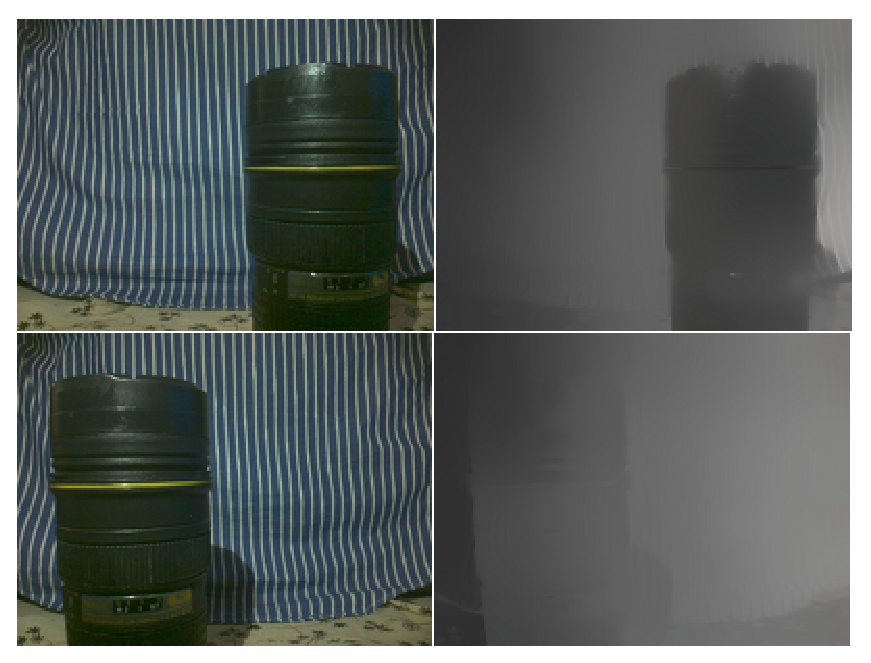
\includegraphics[height=2.0in]{images/merged1}
   \caption{Example set:Upper and lower left: all-in-focus images, and upper and lower right: the corresponding depth map. }
\end{figure}

\begin{figure}[h!]
   \centering
   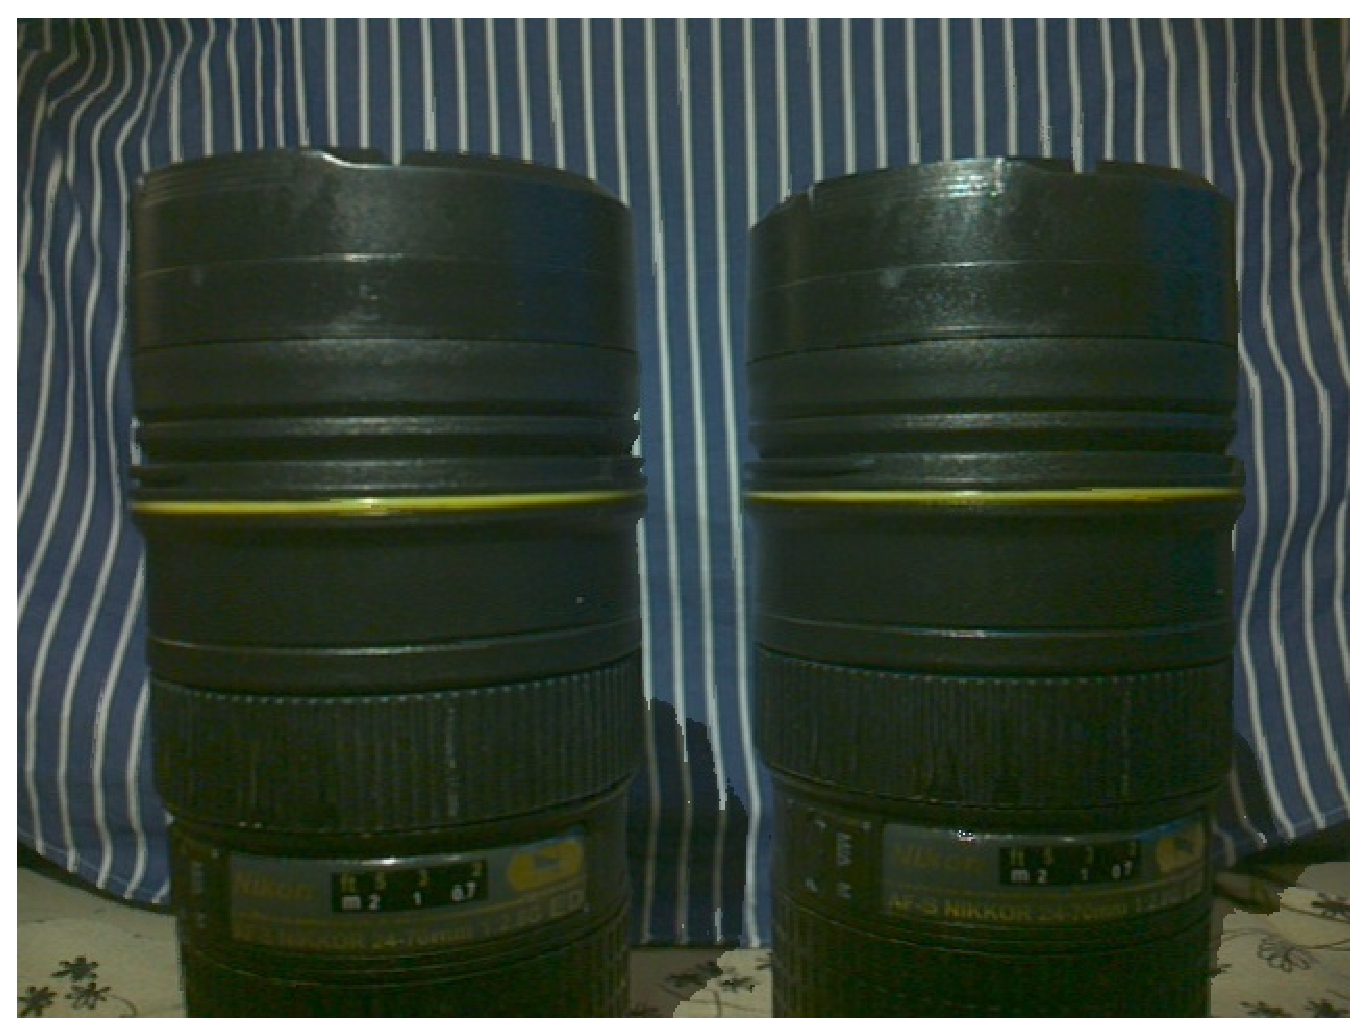
\includegraphics[height=2.0in]{images/merged}
   \caption{Example result: merged image}
\end{figure}

 There is some case that for one pixel, both images have the same depth value. The way we solve this issue now is choosing pixel of one image when this case occurs. 

\subsubsection{Image Depth of Field Image}

\section{Conclusion and Further Works}

Overall, depth from focus provides a good way of achieving an approximate depth map for certain applications.  While the depth map is not perfect for tasks that require clear and definite object borders, like image insertion, it produces very satisfactory all-in-focus images. This is the depth maps are unreliable in places of low texture, but for all-in-focus images, it is difficult to distinguish textureless patches from different depths in the image stack anyway. On the other hand, for object insertion, we can easily have holes in an object filled in by scene from a different depth from the other image.


For the imaging merging part, we need to using image segmentation to solve the ambiguity caused by the case that two images have the same depth value for one pixel. With assistance of image segmentation. we can choose the more likely image to present even if both images have the same depth value. 

\begin{figure}[h!]
   \centering
   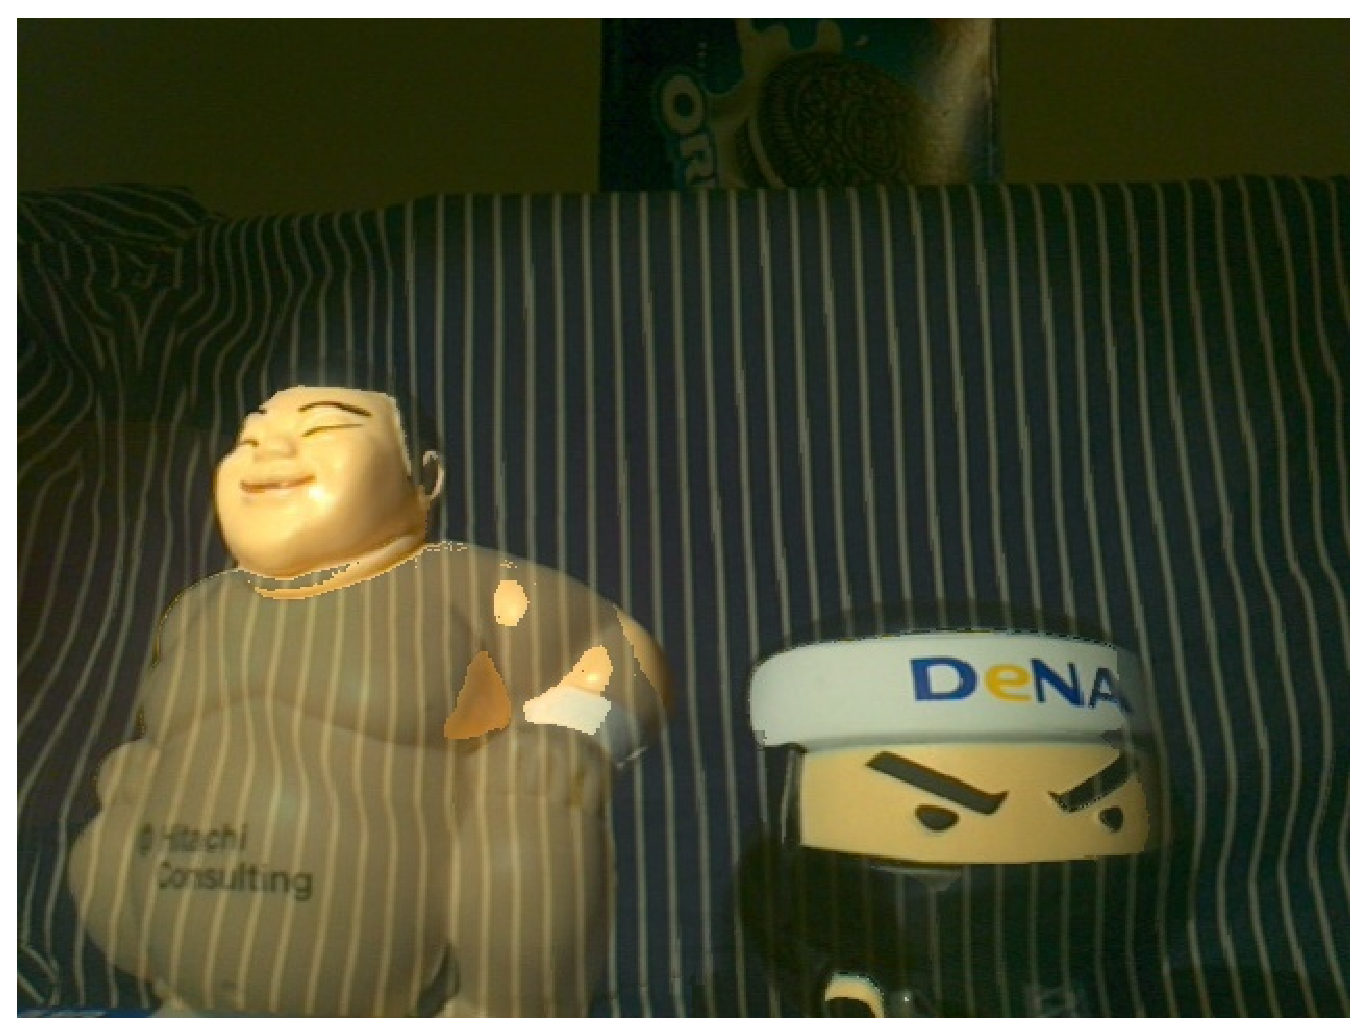
\includegraphics[height=2.0in]{images/faultmerged}
   \caption{Fault image: the semi-transparant parts are the areas have the same depth value in both depth values}
\end{figure}

\subsection{Lighting and Shadows}
One prominent problem with our approach is when the image has strong shadows or specular highlights.  These features produce strong edges in the color space, and thus bilateral filtering may assert a different depth value to these section, even though they should be the same.  This is a difficult problem to solve and is present with other attempts of depth from focus \cite[Grossmann1987] and other unaided image segmentation algorithms.  The best solution to alleviate this problem, if we had more time to implement, is to provide an interface for user feedback and lower the confidence of these segments entirely. 


\section*{Acknowledgements}
(Note: Should acknowledge the CS478 teaching staff for advice and consultation on the project). 


\bibliographystyle{acmsiggraph}
\bibliography{template}
\end{document}
